% !TeX spellcheck = de_DE
\section{\ExercisePrefixEmbeddedC Die Programmiersprache C im Vergleich zu C++}
\label{sec:CVersusCPlusPlus}

Da C++ aus C entstand, sind viele Features von C++ nicht in C enthalten.
Im Folgenden sollen die Hauptunterschiede verdeutlicht werden.

\begin{itemize}
	\item Keine OO-Konzepte (Vererbung, \dots)
    \item Strukturen (\lstinline{struct}) statt Klassen (\lstinline{class})
	\item Keine Templates
	\item Keine Referenzen, nur Zeiger und Werte
	\item Kein \lstinline{new} und \lstinline{delete}, sondern \lstinline{malloc()} und \lstinline{free()} (\lstinline|#include <stdlib.h>|)
	\item Je nach Sprachstandard müssen Variablen am Anfang der Funktion deklariert werden (Standard-Versionen bis einschießlich C99)
	\item Parameterlose Funktionen müssen \lstinline{void} als Parametertyp haben, leere Klammern (bspw. \lstinline{int foo();}) bedeuten, dass beliebige Argumente erlaubt sind.
	\item Keine Streams, stattdessen \lstinline{(f)printf} zur Ausgabe auf Konsole und in Dateien (\verb|#include <stdio.h>|)
	\item Kein \lstinline{bool}-Datentyp, stattdessen wird 0 als \lstinline{false} und alle anderen Zahlen als \lstinline{true} gewertet
	\item Keine Default-Argumente
	\item Keine \lstinline{std::string} Klasse, nur \lstinline{char}-Arrays, die mit dem Nullbyte (\lstinline{'\0'}) abgeschlossen werden.
	\item Keine Namespaces
\end{itemize}

Da einige dieser Punkte sehr entscheidend sind, werden wir auf diese im Detail eingehen.
Wichtig ist hierbei, dass alle im Folgenden vorgestellten Konzepte auch in C++ zur Verfügung stehen.
Die Header der C-Bibliothek sind alle auch in C++ verfügbar.
Möchte man bspw. \lstinline{malloc} nutzen, kann man dies in C++ über \lstinline|#include <stdlib.h>| oder über \lstinline{#include <cstdlib>} (Allgemeines Muster: vorangestelltes 'c' und fehlendes '.h').
Im zweiten Fall sind alle Funktionen im Namensraum \lstinline{std} eingebettet, man muss als \lstinline{std::malloc} nutzen.

\subsection{Kein OO-Konzept}
In C gibt es keine Klassen, weshalb die Programmierung in C eher Pascal statt C++ ähnelt.
Stattdessen gibt es Strukturen (\lstinline{struct}), die mehrere Variablen zu einem Datentyp zusammenfassen, was vergleichbar mit Records in Pascal oder -- allgemein -- mit Klassen ohne Methoden und ohne Vererbung ist.

Die Syntax dafür lautet

  \cpppInputListing{05_c/problems/listings/cintro_structs.c}

Zum Beispiel

  \cpppInputListing{05_c/problems/listings/cintro_structs_ex.c}

Die Sichtbarkeit aller Attribute ist automatisch \lstinline{public}.
Um den definierten \textbf{\lstinline|struct|} als Datentyp zu verwenden, muss man zusätzlich zum Namen das Schlüsselwort \lstinline{struct} angeben:

  \cpppInputListing{05_c/problems/listings/cintro_structs_func.c}

Um den zusätzlichen Schreibaufwand zu vermeiden, wird in der Praxis oft ein \lstinline{typedef} auf den \lstinline{struct} definiert:

  \cpppInputListing{05_c/problems/listings/cintro_structs_typedef.c}

Man kann die Definition eines \lstinline{struct} auch direkt in den \lstinline{typedef} einbauen:

  \cpppInputListing{05_c/problems/listings/cintro_structs_short.c}

\subsection{Kein \lstinline{new} und \lstinline{delete}}

Anstelle von \lstinline{new} und \lstinline{delete} werden die Funktionen \lstinline{malloc} und \lstinline{free} verwendet, um Speicher auf dem Heap zu reservieren.
Diese sind im Header \filename{stdlib.h} deklariert.

  \cpppInputListing{05_c/problems/listings/cintro_mallocfree.c}
  
Der Cast des Ergebnisses von \lstinline|malloc| zu \lstinline|Point*| ist streng genommen nur notwendig, wenn du den gezeigten Code mit einem C++-Compiler kompilierst.
Der C-Compiler nimmt die Konvertierung stillschweigend vor.

\subsection{Ausgabe auf Konsole per \lstinline{printf}}
\cpppSolutionName{microcontroller_c_basics}{micro\-con\-troller\_c\_bas\-ics}

Um Daten auf der Konsole auszugeben, kann die Funktion \lstinline{printf} verwendet werden.
\lstinline{printf} nimmt einen Format-String sowie eine beliebige Anzahl weiterer Argumente entgegen.
Der Format-String legt fest, wie die nachfolgenden Argumente ausgegeben werden.
Mittels \textbackslash n kann man einen Zeilenvorschub erzeugen. Um \lstinline{printf} zu nutzen, muss der Header \filename{stdio.h} eingebunden werden.\footnote{Weitere mögliche Parameter etc. der Funktion \lstinline{printf} findest du unter \url{http://www.cplusplus.com/reference/cstdio/printf/}.}
Der folgende Codeausschnitt zeigt, wie man Zahlen und Zeichen mit \lstinline|printf| ausgeben kann.
Wenn die Variablen \lstinline|i| und \lstinline|c| nicht definiert werden, ist die Aufgabe undefiniert.
Zu beachten ist auch, dass \lstinline|printf| nicht automatisch einen Zeilenumbruch einfügt.
%
  \cpppInputListing{05_c/problems/listings/cintro_printf.c}

Im Folgenden werden wir untersuchen, welche Folgen es hat, wenn man das \enquote{per Konvention} erwartete Null-Byte (\lstinline|'\0'|) entfernt.
In diesem Fall wird der Speicher Byte-weise solange ausgegeben, bis ein Null-Byte angetroffen wird.
\begin{itemize}
\item 
Beginne mit einer leeren \lstinline|main|-Funktion.
\item 
Lege einen Puffer der Größe 8 an:
\begin{lstlisting}
char *buffer = (char*) malloc(8 * sizeof(char));
\end{lstlisting}
\item 
Kopiere mittels \lstinline|strcpy| (aus dem Header \lstinline|string.h|) den String \lstinline|"Hello!!"| in den Puffer:
\begin{lstlisting}
strcpy(buffer, "Hello!!");
\end{lstlisting}
\item 
Nun gib den Inhalt des Puffers mittels \lstinline|printf| aus:
\begin{lstlisting}
printf("%s\n", buffer);
\end{lstlisting}
Wenn du das Programm jetzt kopilierst und ausführst, sollte nur der String \lstinline|Hello!!| erscheinen.
\end{itemize}

\paragraph{Speicher auslesen (Heap)}
Im Folgenden sehen wir uns den Effekt an, den das Weglassen des Nullbytes bewirkt.
Überschreibe zunächst das Null-Byte mit einem beliebigen Zeichen (bspw. \lstinline|'+'|):
\begin{lstlisting}
buffer[strlen(buffer)] = '+'; // or: buffer[7] = '+'
\end{lstlisting}
Die Funktion \lstinline|strlen| liefert die \enquote{gemessene} Länge von \lstinline|buffer| zurück, also die Anzahl an Bytes, bis zum Nullbyte.
Wenn du jetzt den Inhalt des Puffers ausgibst, kann alles passieren (\enquote{Undefined Behavior}).
Die Funktion \lstinline|printf| wird solange den Speicher auslesen, bis sie ein Null-Byte trifft.
Du wirst allerdings nur das neu eingefügte Zeichen (\lstinline|'+'|) zusätzlich sehen, da das Betriebssystem den Heap-Speicher des Programms standardmäßig mit \lstinline|'\0'| überschreibt.

Um einen beeindruckenderen Effekt zu sehen, musst du selber dafür sorgen, dass der Speicher \enquote{sinnvolle} Daten enthält.
Füge dazu den folgenden Code vor dem \lstinline|malloc|-Aufruf von \lstinline|buffer| ein.
\begin{lstlisting}
char *dummyBuffer = (char*) malloc(19 * sizeof(char));
strcpy(dummyBuffer, "AlterTextAlterText");
free(dummyBuffer);
\end{lstlisting}
Wenn du jetzt erneut versuchst, über das Ende von \lstinline|buffer| hinaus zu lesen, solltest du \enquote{Reste} von \lstinline|dummyBuffer| sehen.
Falls du nur \lstinline|Hello!!_| siehst, kann es sein, dass der zweite \lstinline|malloc|-Aufruf einen anderen Speicherbereich zurückliefert als der erste.
Dies kannst du mithilfe der Formatierungsoption \lstinline|%p| prüfen:
\begin{lstlisting}
printf("Address of dummyBuffer: %p\n", dummyBuffer);
printf("Address of buffer:      %p\n", buffer);
\end{lstlisting}
Dieses Experiment zeigt, dass es sehr wichtig ist, bei der Manipulation von C-Strings gut aufzupassen -- 
zahlreiche Sicherheitslücken basieren auf dieser Schwäche!

\paragraph{Speicher auslesen (Konstanten)}
Ändere nun die Art, wie der Puffer allokiert wird, wie folgt:
\begin{lstlisting}
char *myString = "Hello!!";
\end{lstlisting}
Jetzt liegt der Puffer nicht mehr auf dem Heap (wie bei \lstinline|malloc|) sondern im \texttt{data}-Segment.
Wenn du nun versuchst, das Nullbyte von \lstinline|"myString"| zu überschreiben, solltest du einen Speicherzugriffsfehler (\enquote{Segmentation Fault}) erhalten, da Schreibzugriffe in diesem Speicherbereich verboten sind.

\paragraph{Strings einkürzen}
Es ist auch möglich, einen C-String \emph{einzukürzen}, indem man das Null-Byte verschiebt innerhalb des Puffers nach vorne verschiebt.
\begin{itemize}
\item
Verwende den Code aus dem vorherigen Abschnitt und diejenige Zeile an, in der der Puffer manipuliert wird.
Statt \lstinline|'_'| an Index 5 zu platzieren, platziere jetzt das Null-Byte (\lstinline|'\0'|) an Index 2.
\item 
Bei der Ausführung sollte jetzt nur noch \texttt{He} ausgegeben werden.
\end{itemize}

\subsection{Strings zusammenbauen}

Die Funktion \lstinline{sprintf} dient dazu, formatierte Strings zusammenzusetzen und ist syntaktisch eng mit der Funktion \lstinline{printf} verwandt.\footnote{Weitere mögliche Parameter etc. der Funktion \lstinline{sprintf} findest du unter \url{http://www.cplusplus.com/reference/cstdio/sprintf/}.}
%
\begin{itemize}
\item
Beginne mit einer leeren \lstinline|main|-Funktion.
\item 
Lege erneut einen Puffer auf dem Heap an:

\begin{minipage}{.96\textwidth}
\begin{lstlisting}
char *buffer = (char*) malloc(100 * sizeof(char));
\end{lstlisting}
\end{minipage}

\item 
Verwende den folgenden Aufruf, um einen Gruß mittels \lstinline|sprintf| zusammenzusetzen.
Lege dazu im Vorfeld eine Variable \lstinline|name| an.
\begin{lstlisting}
sprintf(buffer, "Hello, %s!\n", name);
\end{lstlisting}
\item 
Den so gefüllten Puffer gibst du wie gewohnt über \lstinline|printf| aus:
\begin{lstlisting}
printf(buffer);
\end{lstlisting}
\item 
Die Funktion \lstinline|sprintf| kann natürlich auch zur Ausgabe (bspw.) von Zahlen und Zeichen genutzt werden:
\begin{lstlisting}
sprintf(buffer, "c = %c, i = %3d", c, i);
\end{lstlisting}
\end{itemize}
Beachte auch hier, dass der Puffer auf dem Heap (statt im \texttt{data}-Segment) liegen muss, damit die Funktion \lstinline|sprintf| hineinschreiben kann.
Andernfalls erhältst du einen Segmentation Fault.

\subsection{Zahlen formatiert ausgeben}
\label{sec:CFormatNumbers}
Schreibe ein C-Programm, welches alle geraden Zahlen von 0 bis 200 formatiert ausgibt.
Die Formatierung soll entsprechend dem Beispiel erfolgen:
%
  \cpppInputListing{05_c/problems/listings/cintro_format.c}
%
Mache die Spaltenzahl und Spaltenbreite mithilfe von Variablen konfigurierbar, sodass es auch leicht möglich ist, 15 Spalten und/oder Zahlen bis \numprint{10 000} auszugeben.

\subsection{structs und unions}


Als Beispiel sehen wir uns dazu eine Struktur für die ARGB-Farbkodierung an (mit alpha-, rot-, grün- und blauem Farbkanal). 

\cpppInputListing{05_c/problems/listings/channels_struct.c}

%union color beispiel interaktiv gestalten. Folien Willert 02b seite 9-11

Neben structs gibt es auch unions, welche syntaktisch ähnlich sind.
Der Unterschied ist, dass hier die einzelnen Felder vereint werden und sich den gleichen Speicherplatz teilen. 
Verändert man also eine der Variable, ändert sich der gemeinschaftlich genutzte Speicherplatz und der Wert der anderen Variablen entsprechend. 
Demnach ist eine Vereinigung dann sinnvoll, wenn der Wert einer Variablen unabhängig vom Typ gleichviel Speicherplatz benötigt und im selben Speicherbereich abgelegt werden soll.


Die ARGB-Farbcodierung lässt sich statt in 4 einzelnen Variablen auch als eine einzige Integer Variable schreiben, weshalb wir hier eine \lstinline{union} verwenden können.



\cpppInputListing{05_c/problems/listings/union.c}


Übernehme nun den obigen Code in dein eigenes Projekt und lass dir in der \lstinline{main}-Funktion die Größe der Variable \lstinline{c}, den Inhalt der Variablen in der \lstinline{union}, sowie die Speicherstellen aller einzelnen Variablen des structs sowie der Integer Variablen mit Hilfe von \lstinline{printf} ausgeben. 
Was stellst du fest? 
Die Darstellung des Speichers in Abbildung \ref{fig:color_channels} sollte dir weiterhelfen.

\begin{figure}[!htb]
	\centering
	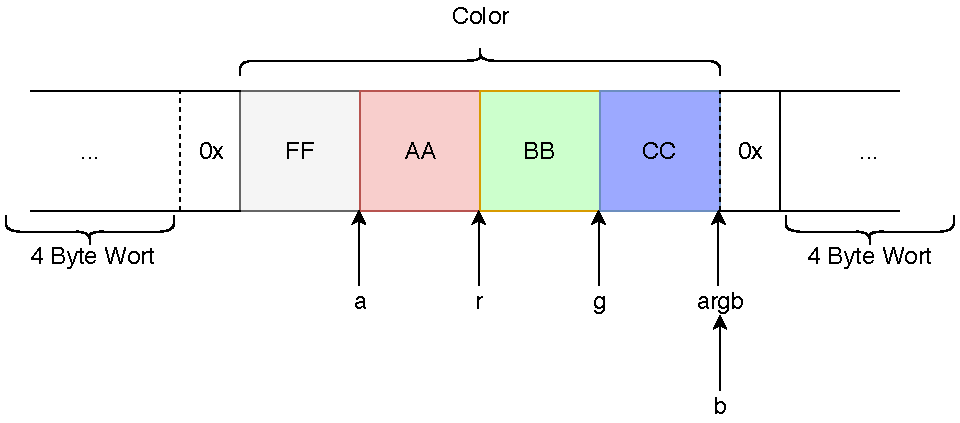
\includegraphics[width=0.6\textwidth]{./05_c/figures/Color_Channels.pdf}
	\caption{Union Color im Speicher}
	\label{fig:color_channels}
\end{figure} 

\hints{
	\item Mit \lstinline{\%x} kannst du Zahlen in Hexadezimal formatieren.
	
}


\subsection{Bit-Operatoren in C (und C++)}
\label{task:bitops}

In dieser Aufgabe machst du dich mit den Bit-Operatoren (\lstinline{&, |, ~, >>, <<}) in C vertraut.
Alle Operatoren können exakt gleich in C++ verwendet werden.
Bit-Operatoren sind für ganzzahlige Typen definiert (bspw. \lstinline|(unsigned) int|, \lstinline|(unsigned) char|).
Ein Bit-Operator bezieht sich dabei auf jedes einzelne Bit.
Im Gegensatz dazu beziehen sich logische Operatoren (\lstinline{||, &&}) immer auf den gesamten Wert.

Zum Experimentieren stellen wir dir eine Vorlage zur Verfügung: \url{https://github.com/Echtzeitsysteme/tud-cppp/blob/master/exercises/templates/BitAndLogicOperations/BitAndLogicOperations.c}.
Die Funktion \lstinline|fmt| wandelt ein Byte in einen String um, der das Bit-Muster darstellt.
Zum Beispiel ist die Ausgabe von \lstinline|fmt(23)| der String \lstinline|"0b00010111"| ($19 = 1 + 2 + 4 + 16$).
\begin{itemize}
\item 
Fülle zunächst die mit \lstinline|// TODO implement me| gekennzeichneten Zeilen aus, sodass die Ausgabe korrekt ist.
Beispiele sind für \texttt{NEG} und \texttt{NOT} gegeben.

Stelle sicher, dass deine Ergebnisse für \lstinline|a = 23, b = 3| mit den erwarteten Ergebnisse in folgender Tabelle übereinstimmen\\[1ex]
\begin{center}
\begin{tabular}{lr}
\toprule
\textbf{Ausdruck} & \textbf{Ergebnis}\\
\midrule
\texttt{a AND b} & 3\\
\texttt{a OR b} & 23\\
\texttt{a XOR b} & 20\\
\midrule
\texttt{a RIGHT s} & 5\\
\texttt{a LEFT s} & 92\\
\bottomrule
\end{tabular}
\end{center}

Die folgende Tabelle enthält die erwarteten Ergebnisse der logischen Operatoren für alle Wertkombinationen von \lstinline|a| und \lstinline|b|.
Mit \texttt{IMP} ist Implikation gemeint ($\Rightarrow$) und mit \texttt{BIIMP} ist Biimplikation/Äquivalenz gemeint ($\Leftrightarrow$).\\[1ex]
\begin{center}
\begin{tabular}{lrrrr}
    \toprule
    \textbf{Ausdruck} & \multicolumn{4}{c}{\textbf{Ergebnis}}\\
    & \lstinline|a=1,b=1| & \lstinline|a=1, b=0| & \lstinline|a=0, b=1| & \lstinline|a=0, b=0|\\
    \midrule
    \texttt{a LAND s}  & 1  & 0& 0& 0\\
    \texttt{a LOR s}   & 1  & 1& 1& 0\\
    \texttt{a XOR s}   & 0  & 1& 1& 0\\
    \texttt{a IMP s}   & 1  & 0& 1& 1\\
    \texttt{a BIIMP s} & 1  & 0& 0& 1\\
    \bottomrule
\end{tabular}
\end{center}
\item 
Im Allgemeinen entspricht eine Verschiebung nach links/rechts einer Multiplikation mit/Division durch 2.
Dazu werden jeweils von rechts/links 0-Bits eingeschoben.
Unter welchen Umständen gilt dies nicht mehr?
Was passiert, wenn du den Datentyp von \lstinline|a| auf \lstinline|unsigned char| setzt?
Beobachte auch, ob das angezeigte Bitmuster mit dem ausgegebenen Wert übereinstimmt.
% << Überlauf 127/255 zu 0, aber der Ausdruck "a << s" wird automatisch in den nächsthöheren Typ konvertiert!
% >> Anrunden bei nicht durch 2^s teilbaren Werten
\item 
Ändere den Wert der Variablen \lstinline|a| in \lstinline|-1|.
Was passiert bei einem Rechts-Shift?
Was bei einem Links-Shift?
Wie unterscheidet sich das Verhalten im Vergleich zu positivem \lstinline|a|?
% Es werden '1' statt '0' eingeschoben
\item 
Ändere den Wert von \lstinline|s| zu -1.
Wie sieht das Ergebnis des Rechts-/Links-Shifts aus?
Ein Shift um einen negativen Wert ist \enquote{Undefined Behavior}.
Welche Ergebnisse sind demnach erlaubt?
\end{itemize}

\subsection{C++-Aufgaben nachprogrammieren \optional}

\optionaltextbox

Dies ist eine freie Aufgabe, in der du versuchst, Programme der vergangenen Tage in reinem C auszudrücken.
Der Schwierigkeitsgrad ist dabei sehr unterschiedlich!

\paragraph{Niedrigerer Schwierigkeitsgrad}
\begin{itemize}
\item
\textbf{Sternen- oder Buchstabenmuster} ausgeben (\ref{sec:basics}):
Diese Aufgabe ist sehr ähnlich zu \ref{sec:CFormatNumbers}.

\item
\textbf{Werte analysieren} und mit \textbf{Arrays} arbeiten (\ref{sec:pointers} und \ref{sec:arrays}):
Abgesehen von der fehlenden Unterstützung für Referenzen sollten die Ergebnisse sich nicht unterscheiden.

\item
\textbf{Funktionszeiger} (\ref{sec:functional} und \ref{sec:callbacks}):
Funktionszeiger in C arbeiten genauso wie Funktionszeiger in C++.
Du kannst dies testen, indem du die Programmlogik der vorigen Aufgabe in eine separate Funktion auslagerst, die neben der Spaltenbreite und Obergrenze der anzuzeigenden Zahlen zusätzlich einen Funktionszeiger-Parameter hat, der festlegt, was mit der jeweiligen Zahl vor der Ausgabe geschehen soll (bspw. verdoppeln, quadrieren).
\end{itemize}

\paragraph{Höherer Schwierigkeitsgrad}
\begin{itemize}
\item
\textbf{\lstinline|Vector|} (\ref{sec:overloading}): C bietet keine Objektorientierung, aber du kannst eine \lstinline|struct| zur Datenhaltung anlegen und die Methoden der Klasse als Funktionen realisieren, deren Namen bspw. immer mit dem Präfix \lstinline|Vector_| beginnen und die als zusätzlichen Parameter einen Pointer auf eine \lstinline|Vector|-\lstinline|struct| erhalten.

\item 
\textbf{Verkettete Listen} (\ref{sec:linkedList}):
Die reinen Datenstrukturen für die Liste (\lstinline|List|) und für Listenelemente (\lstinline|ListItem|) lassen sich als \lstinline|struct| abbilden.
Methoden kannst du wieder auf Funktionen mit Namenskonvention und zusätzlichem Pointer-Parameter abbilden.

\item
\textbf{Generischer Vektor und Liste} (\ref{sec:genericVector} und \ref{sec:genericLinkedList}):
Auch wenn es in C keinen eingebauten Mechanismus wie die C++-Templates gibt, kannst du die \lstinline|Vector| und \lstinline|List|-Klasse generisch machen, indem du die Einträge des Vektors bzw. den \lstinline|content| der \lstinline|ListItems| als \lstinline|void*| deklarierst.

\item
\textbf{Eigene \lstinline|Array|-Klasse} (\ref{sec:customArrays}):
Ebenso wie bei generischem Vektor und Liste kannst du natürlich auch deine eigene \lstinline|Array|-Klasse schreiben.
\end{itemize}
